\documentclass[journal]{IEEEtran}
\IEEEoverridecommandlockouts
% The preceding line is only needed to identify funding in the first footnote. If that is unneeded, please comment it out.
%Template version as of 6/27/2024

\usepackage{cite}
\usepackage{amsmath,amssymb,amsfonts}
\usepackage{algorithmic}
\usepackage{graphicx}
\usepackage{float}
\usepackage{subcaption}
\usepackage{textcomp}
\usepackage{xcolor}
\usepackage{hyperref}
\def\BibTeX{{\rm B\kern-.05em{\sc i\kern-.025em b}\kern-.08em
    T\kern-.1667em\lower.7ex\hbox{E}\kern-.125emX}}
\begin{document}

\title{HVAC waste detection based on rapid temperature changes\\
{\footnotesize Internet of Things Project - Year 2023-2024}}

\author{\IEEEauthorblockN{Leonardo Dessì}
\IEEEauthorblockA{\\\textit{Università di Bologna} \\
Bologna, Italy \\
leonardo.dessi@studio.unibo.it\\
Student ID number: 0001141270}
}

\maketitle

\begin{abstract}
This paper presents a comprehensive Internet of Things (IoT) solution for monitoring and controlling HVAC systems with intelligent energy waste detection capabilities. The system integrates Arduino-based sensors, MQTT communication protocols, machine learning algorithms, and real-time data visualization to provide automated detection of energy wastage through rapid temperature changes. The architecture comprises four main components: firmware for IoT devices, a data proxy for communication bridging, a data analytics engine with predictive capabilities, and visualization dashboards. The system employs ARIMA-based temperature prediction models to forecast indoor temperature patterns and automatically detects potential energy waste scenarios when HVAC systems are active. Performance evaluation demonstrates the system's effectiveness in real-time monitoring, prediction accuracy across multiple time horizons, and reliable alert generation for energy optimization.
\end{abstract}

\begin{IEEEkeywords}
Internet of Things, HVAC monitoring, energy efficiency, machine learning, ARIMA prediction, MQTT communication, InfluxDB, temperature forecasting, energy waste detection
\end{IEEEkeywords}

\section{Introduction}

Energy efficiency in building management systems has become increasingly critical due to rising energy costs and environmental concerns. Heating, Ventilation, and Air Conditioning (HVAC) systems typically account for 38\% of total building energy consumption, making them prime targets for optimization strategies\cite{GONZALEZTORRES2022626}. Traditional HVAC control systems often operate on simple thermostatic controls without considering external environmental factors, occupancy patterns, or predictive analytics, leading to significant energy waste.

The rapid advancement of Internet of Things (IoT) technologies presents unprecedented opportunities for intelligent building management systems. IoT-enabled sensors can provide continuous monitoring of environmental conditions, while machine learning algorithms can analyze patterns and predict future states to optimize system operation. The integration of real-time data analytics with predictive modeling enables proactive energy management rather than reactive control.

This project addresses the challenge of HVAC energy waste detection through the development of a comprehensive IoT monitoring system. The system focuses specifically on detecting energy waste scenarios based on rapid temperature changes that indicate inefficient HVAC operation. By combining real-time sensor data with predictive analytics, the system can identify situations where HVAC systems are operating unnecessarily or inefficiently.

The primary objectives of this work are: (1) to develop a scalable IoT architecture for continuous HVAC monitoring, (2) to implement time-series forecasting models for temperature prediction and anomaly detection, (3) to create an integrated communication framework using MQTT protocols for real-time device control, and (4) to provide comprehensive visualization and alerting capabilities for system operators.

The system's innovation resides in its comprehensive approach to energy waste detection, which integrates diverse data sources such as indoor and outdoor temperature sensors, external weather APIs, and HVAC system status information to facilitate intelligent inference of energy consumption patterns. The use of ARIMA-based forecasting models enables the system to predict temperature trends and identify deviations that indicate potential waste scenarios.

\section{Project's Architecture}
\begin{figure*}[ht]
    \centering
    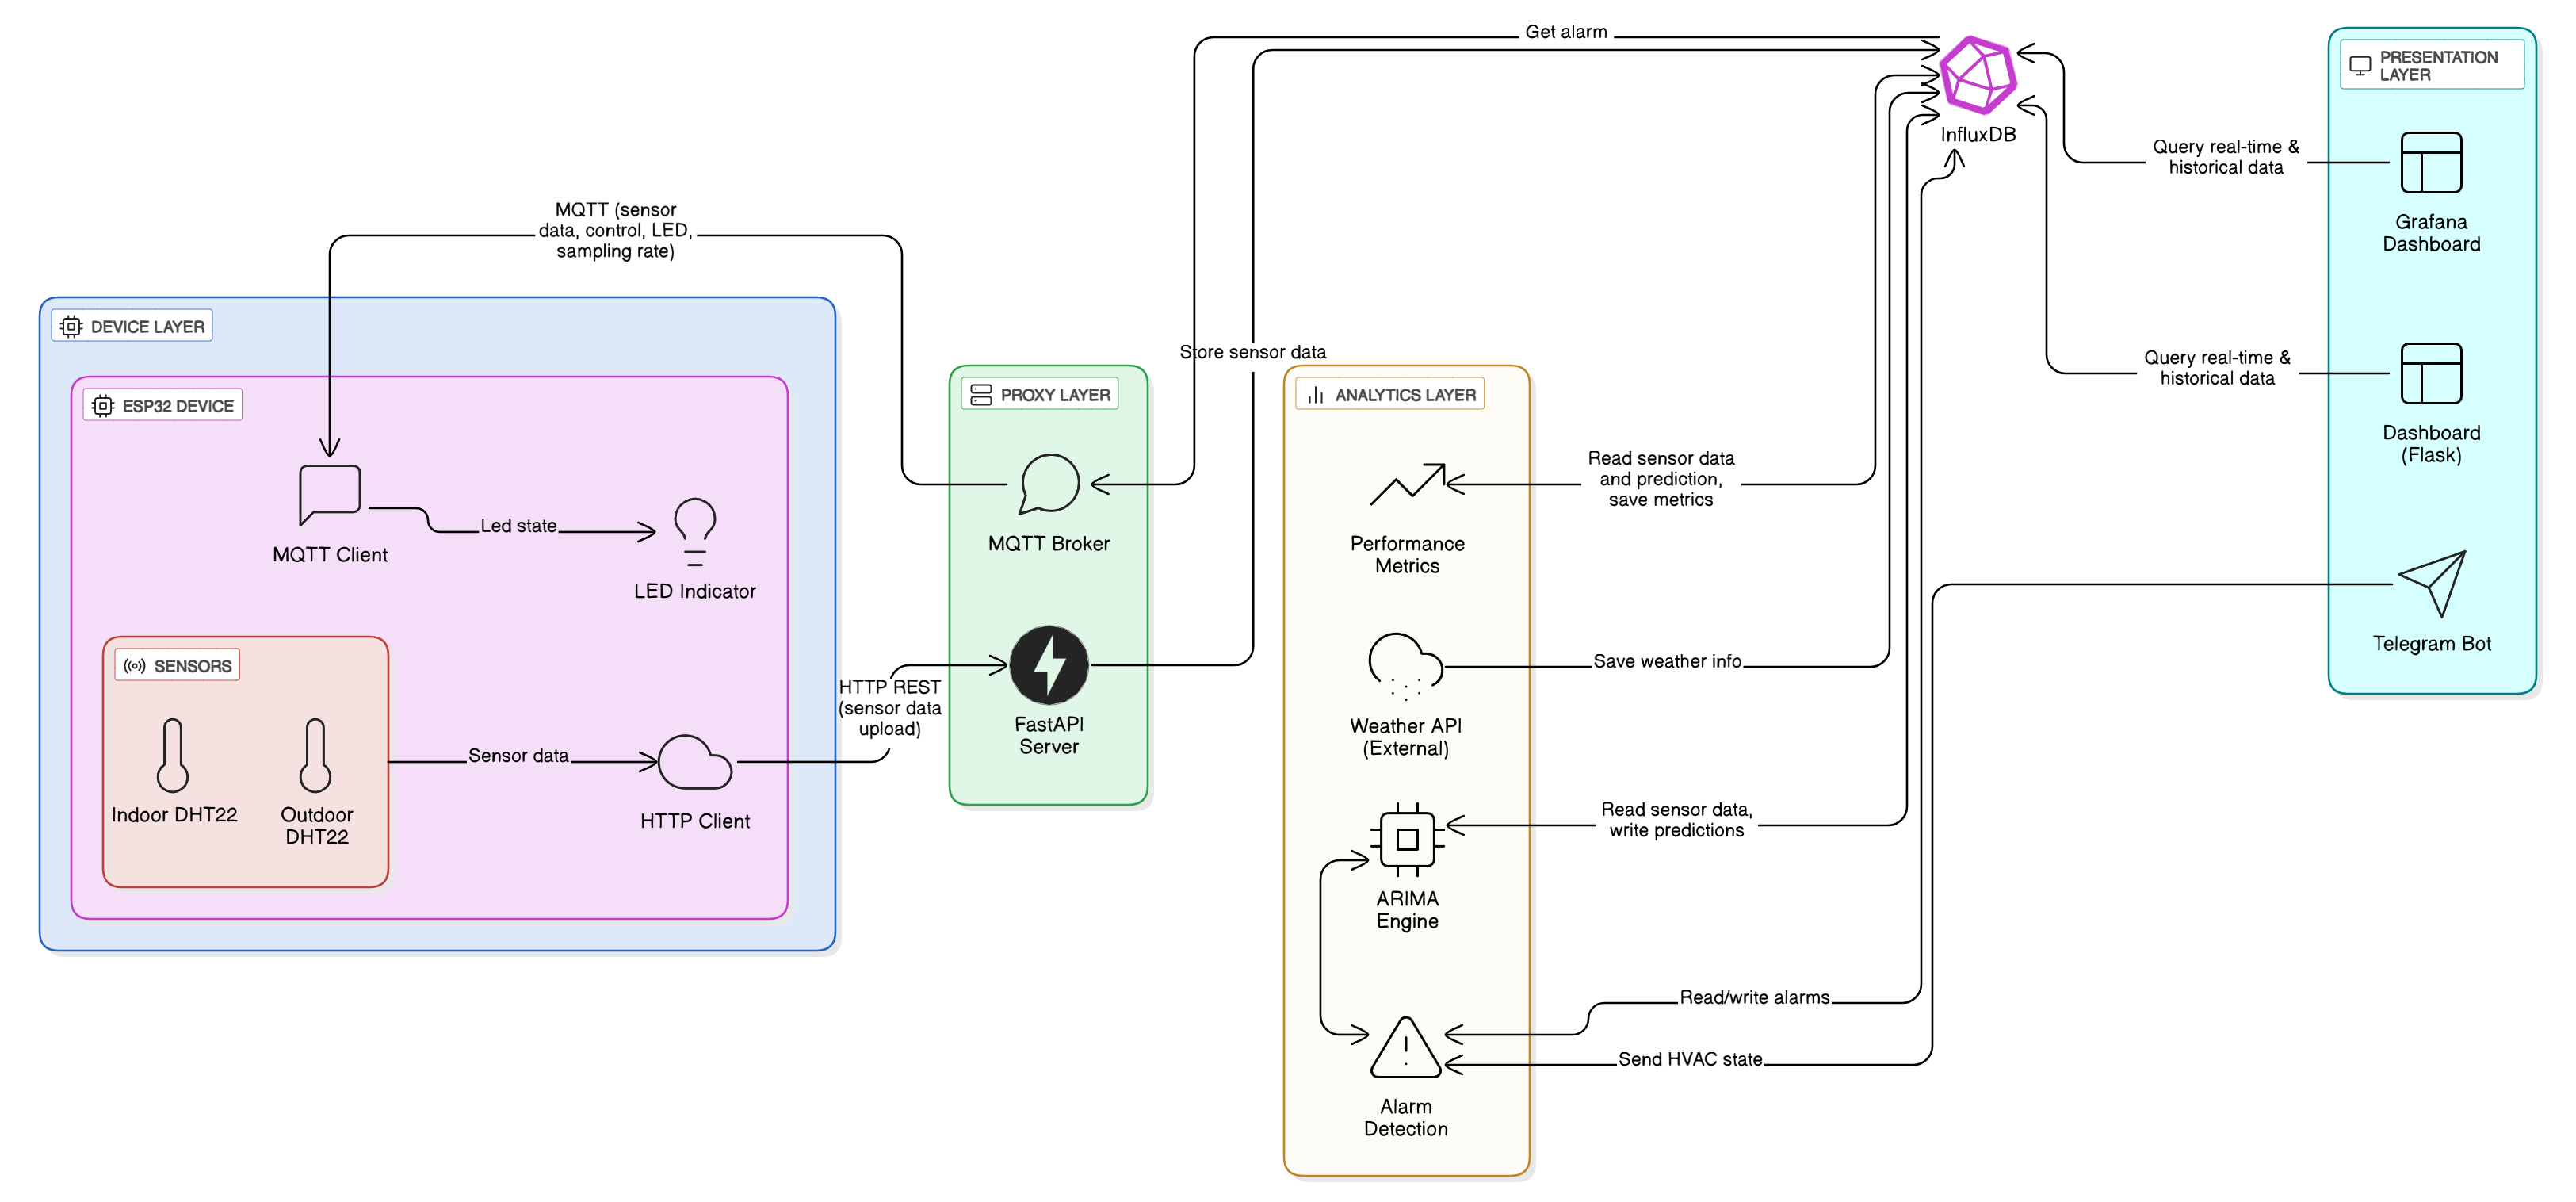
\includegraphics[width=1\textwidth]{image/architettura.png}
    \caption{System Architecture}
    \label{fig:architecture}
\end{figure*}

The IoT HVAC monitoring system is designed as a comprehensive, end-to-end solution that emphasizes modularity and scalability. It provides an integrated infrastructure for environmental sensing and control, effectively linking physical devices with advanced data analytics and user-facing interfaces.

\subsection{System Overview}

The architecture adopts a \textbf{hub-and-spoke model}, in which IoT devices collect environmental data and transmit it to a centralized proxy. The system supports \textbf{bidirectional communication}: data is sent from sensors to the proxy, and control commands are issued in the reverse direction. Notably, data from the ESP32 devices is transmitted via \textbf{HTTP}, while control commands from the proxy to the ESP32 are delivered using the \textbf{MQTT protocol}.

The data flow begins at the sensor level, progresses through a communication layer managed by the data proxy, and is then forwarded to storage and analytics layers. Finally, data is rendered through user-facing presentation layers. Figure~\ref{fig:architecture} illustrates these components and their interconnections.

\subsection{Hardware Components}

The system's hardware foundation consists of \textbf{ESP32 microcontrollers}, which function as the edge computing units. Each ESP32 interfaces with two \textbf{DHT22 sensors} to measure temperature and humidity in both indoor and outdoor settings, facilitating context-aware decision-making. An \textbf{LED indicator} connected to the ESP32 provides real-time visual feedback regarding system status.

\subsection{Software Components}

The software architecture follows a \textbf{multi-tiered design} to separate concerns effectively. The base layer comprises \textbf{Arduino-compatible firmware} running on the ESP32, which manages sensor readings and network communication. A \textbf{data proxy layer}, implemented in Python with FastAPI, bridges edge devices and higher-order services. This proxy conducts initial data validation, exposes a GUI interface, and forwards control commands.

An \textbf{analytics backend} processes time-series data using pipelines that incorporate prediction models and system diagnostics. This backend leverages \textbf{InfluxDB} for efficient storage of temporal data. Visualization is achieved through web technologies, while a \textbf{Telegram bot} provides a mobile access point. The system also integrates \textbf{weather APIs} and cloud services via \textbf{InfluxDB Cloud (EU Central)}.

\subsection{Network Topology}

The network employs a \textbf{hybrid topology} for connectivity. The ESP32 devices use onboard \textbf{Wi-Fi} to connect to a local network. \textbf{HTTP} is employed for transmitting sensor data from the ESP32 to the proxy, using POST requests with JSON payloads. In contrast, \textbf{MQTT} is used exclusively for sending control commands from the proxy back to the ESP32 devices.

\subsection{Data Flow}

Environmental data originates at the \textbf{DHT22 sensors}, which record measurements at user-defined intervals (default: 5 seconds). The ESP32 formats these readings into \textbf{JSON} and transmits them to the proxy via \textbf{HTTP POST} requests, including timestamps for latency analysis. The proxy validates and forwards the data to \textbf{InfluxDB} for storage.

The \textbf{Analytics Backend} retrieves stored data, performs aggregations and transformations, and generates short-term temperature forecasts (1, 10, 20, and 30 minutes). Forecast accuracy is continuously assessed against real readings. If anomalies indicative of energy inefficiency are detected, commands are issued through \textbf{MQTT topics} to trigger system responses, completing the sense-analyze-act cycle.

\subsection{Block Architecture}

From a block-level perspective, the system exhibits clear functional stratification:

\begin{itemize}
    \item \textbf{Edge Layer}: ESP32 and sensors.
    \item \textbf{Communication Layer}: HTTP (sensor data to proxy), MQTT (commands to devices).
    \item \textbf{Storage Layer}: InfluxDB for time-series data.
    \item \textbf{Processing Layer}: Analytics and forecasting.
    \item \textbf{Presentation Layer}: Dashboards, GUIs, Telegram bot.
    \item \textbf{Integration Layer}: External APIs and cloud services.
\end{itemize}


\section{Project Implementation}

The implementation of the IoT-based HVAC monitoring system integrates embedded hardware with a multi-layered software stack, resulting in a robust, scalable, and feature-rich architecture for environmental monitoring and energy efficiency analysis.

\subsection{Hardware Configuration}

\begin{figure}[ht]
    \centering
    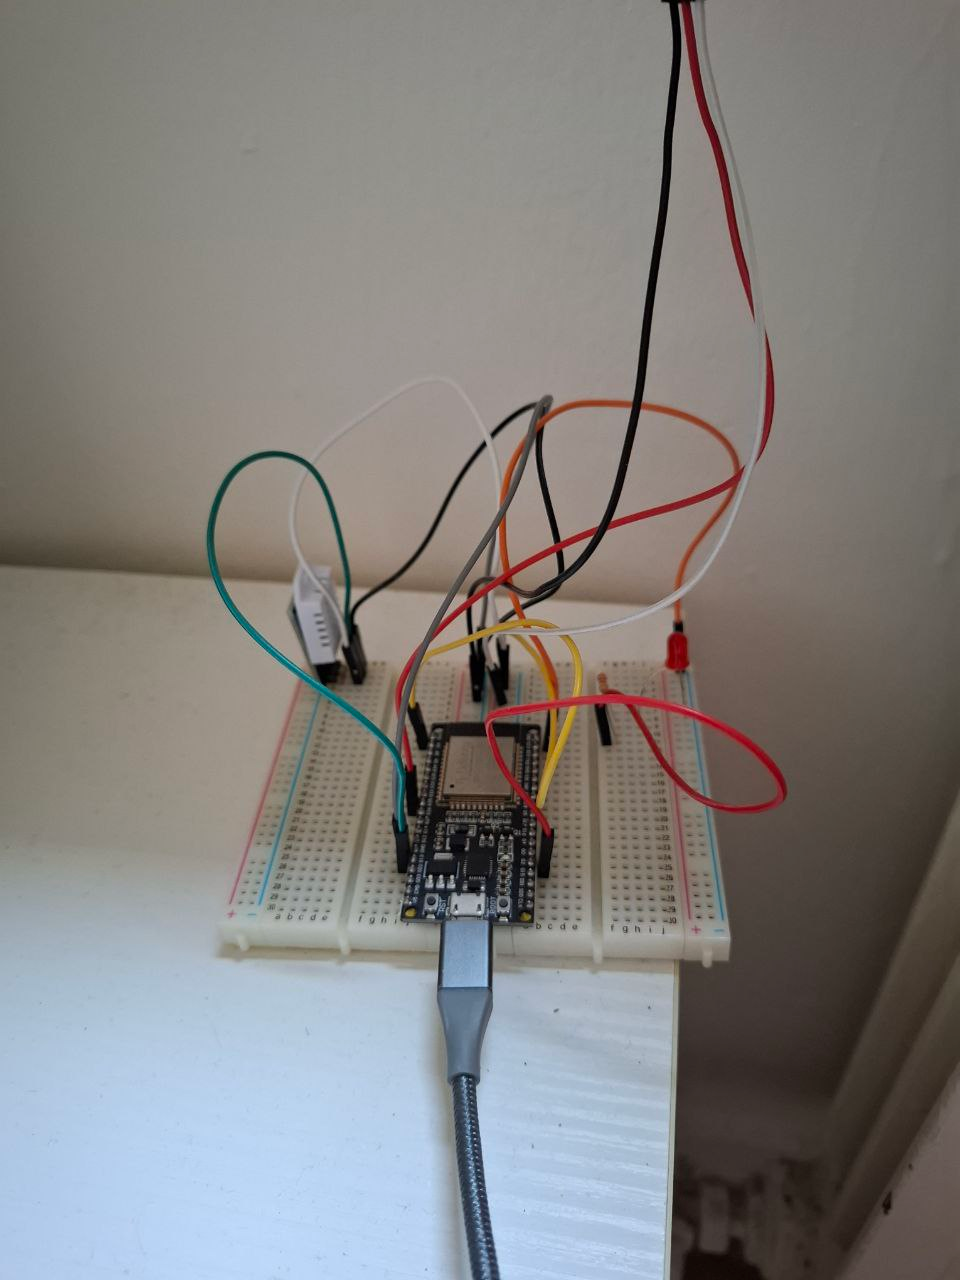
\includegraphics[width=0.49\linewidth]{image/esp32_photo.png}\hfill
    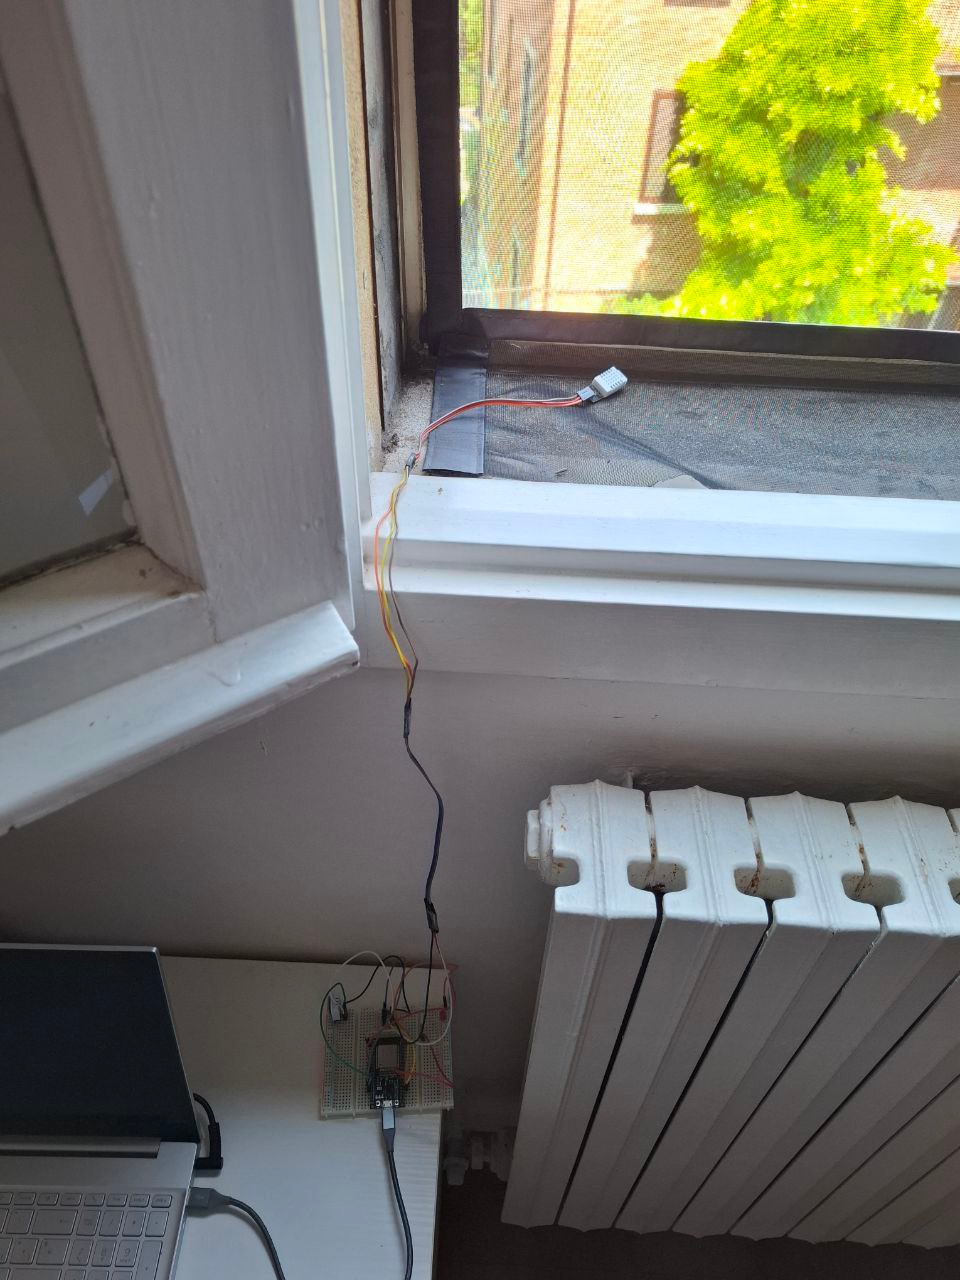
\includegraphics[width=0.49\linewidth]{image/esp32_photo2.png}
    \caption{ESP32 configuration}
    \label{fig:esp32-configuration}
\end{figure}

At the core of the hardware setup lies the \textbf{ESP32 microcontroller}. Two \textbf{DHT22 sensors} are interfaced with the ESP32 to provide temperature and humidity measurements. The indoor sensor is connected to pin 13, while the outdoor sensor is connected to pin 25. Additionally, an \textbf{LED indicator} is connected to pin 2 to offer immediate visual feedback regarding the alarm state(if the led is on a waste is detected), thereby facilitating rapid diagnostics in the absence of a graphical interface.

The ESP32 establishes a connection to the local Wi-Fi network using credentials embedded within its firmware and maintains concurrent connections with both the HTTP server and the MQTT broker. To support high-precision time-series analytics, the system implements \textbf{NTP-based time synchronization} during the boot sequence and at predefined intervals.

\begin{figure}[H]
    \centering
    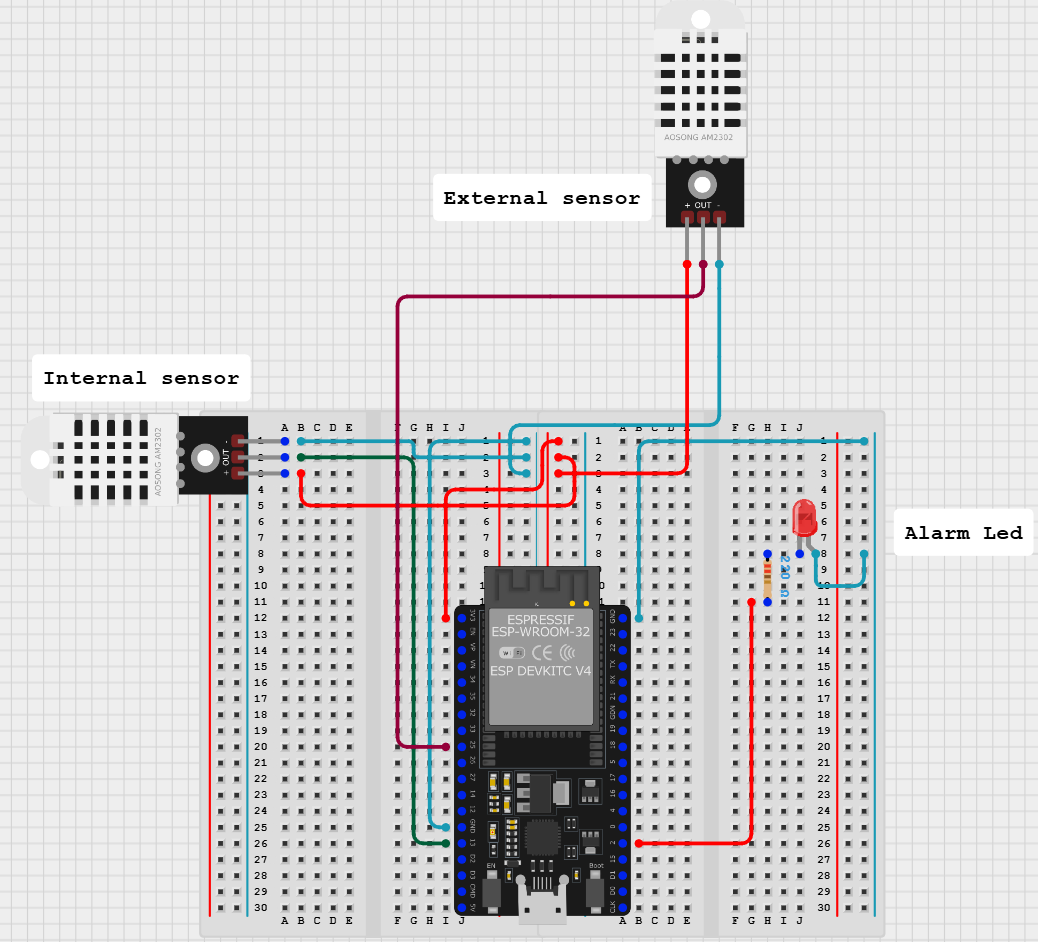
\includegraphics[width=1\linewidth]{image/circuit.png}
    \caption{Circuit scheme}
    \label{fig:circuit-configuration}
\end{figure}

\subsection{Software Architecture}

The software implementation spans several programming languages and frameworks, each selected to address specific functional requirements of the system. The ESP32 firmware is developed in \textbf{Arduino/C++}, responsible for managing sensor data acquisition, wireless communication, and MQTT-based messaging for command reception and data publishing.

The \textbf{Data Proxy} is implemented in \textbf{Python} using the \textbf{FastAPI} framework. It exposes efficient asynchronous endpoints for ingesting sensor data and features a \textbf{Tkinter-based GUI} for real-time monitoring and control (it can send MQTT message to ESP32). The \textbf{Analytics Backend}, also developed in Python, utilizes the \textbf{Flask} framework to serve dashboards and RESTful APIs. This backend incorporates \textbf{NumPy} and \textbf{Pandas} for data manipulation, and ARIMA for predictive modeling. \textbf{Threading mechanisms} enable concurrent execution of computational tasks, thereby enhancing responsiveness and system throughput.

For client-side visualization, the system employs \textbf{JavaScript} with the \textbf{Chart.js} library, embedded within responsive \textbf{HTML/CSS} templates. Data visualizations are updated in real-time through periodic \textbf{HTTP requests} to the exposed Flask API. A dedicated \textbf{Telegram bot}, developed using the \textbf{python-telegram-bot} library, enables mobile interaction with the system via Telegram's API. The Telegram bot is used to manually set the status of HVAC. If the HVAC status is on the alarm are generated, else they are not generated. It supports asynchronous message handling and offers an \textbf{inline keyboard interface} for intuitive control. Time-series database operations are facilitated using \textbf{InfluxDB Python client libraries}, with advanced querying performed using the \textbf{Flux} language.

\subsection{Data Processing Pipeline}

The system's data pipeline transforms raw sensor inputs into actionable insights through a structured sequence of operations. Timestamps are assigned at the point of acquisition on the ESP32 to ensure accurate latency tracking. Incoming data undergoes validation and cleaning procedures to filter out anomalous values that could indicate sensor malfunction. Following standardization into 30-second aggregation windows, validated data is stored in measurement-specific \textbf{InfluxDB} buckets.

\textbf{Flux queries} are utilized for temporal aggregation and pivot operations, preparing the data for downstream analytics. The pipeline calculates statistical correlations between indoor and outdoor temperatures to infer potential inefficiencies in energy usage.

A central component of the pipeline is its \textbf{predictive analytics} capability. Historical temperature data is used to fit ARIMA model that forecast indoor temperatures at future time horizons of 1, 10, 20, and 30 minutes. These forecasts enable anticipatory HVAC control strategies. Model performance is continuously evaluated using metrics such as \textbf{Mean Absolute Error (MAE)}, \textbf{Mean Squared Error (MSE)}, and \textbf{Root Mean Squared Error (RMSE)}, which are exposed through a dedicated dashboard. In addition, the system detects potential energy waste by analyzing indoor-outdoor temperature differentials and can trigger LED-based alerts via MQTT when significant inefficiencies are identified.

\subsection{Communication Protocols}

The system employs a hybrid communication model, using protocols suited to the specific needs of data flow and control. \textbf{MQTT} is used exclusively for transmitting control commands and receiving real-time status updates. The MQTT broker operates on a local server and enforces authentication through credentials configured in the ESP32 firmware. Key MQTT topics include \texttt{hvac/control} (system activation), \texttt{hvac/led} (indicator control), and \texttt{hvac/sampling\_rate} (sensor frequency adjustment).


\textbf{HTTP/REST} complements MQTT by facilitating structured data exchange. The Data Proxy provides RESTful endpoints for data ingestion, while the Analytics Backend exposes endpoints for historical data retrieval. All API communications are conducted using standardized \textbf{JSON} formats. For database access, the system leverages both the \textbf{InfluxDB REST API} and specialized client libraries, with data insertion and query operations conducted using the \textbf{Write API} and \textbf{Flux query language}, respectively.

\begin{figure*}[t]\renewcommand{\thefigure}{5}
    \centering
    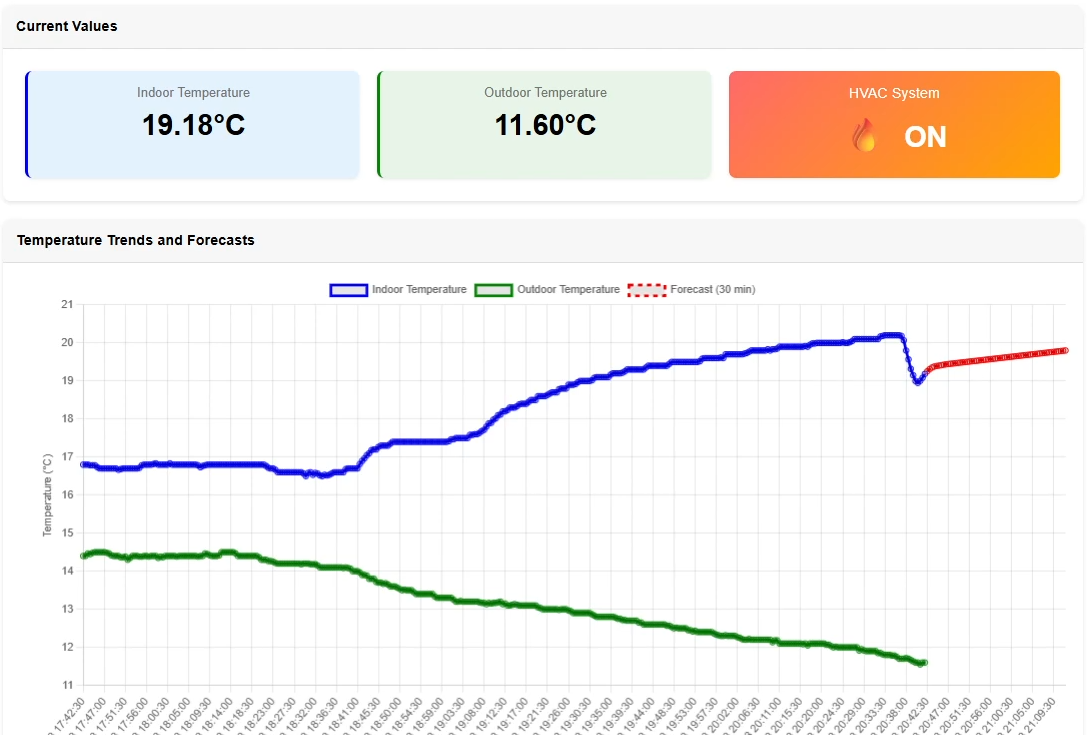
\includegraphics[width=0.49\linewidth]{image/dashboard.png}\hfill
    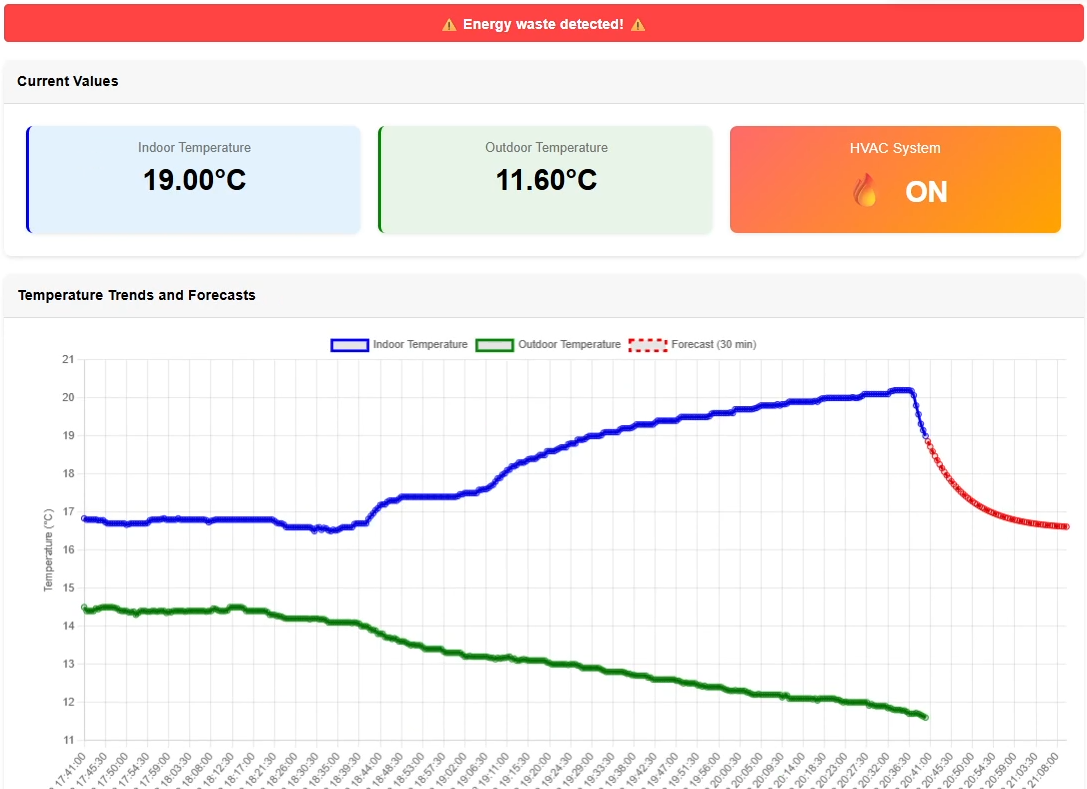
\includegraphics[width=0.49\linewidth]{image/dashboard_alarm.png}
    \caption{Dashboard with and without energy waste detected}
    \label{fig:dashboard}
\end{figure*}

\subsection{Prediction of temperatures}
The core of the system's predictive analytics capability is realized through a machine learning-based temperature forecasting module, which leverages an ARIMA (AutoRegressive Integrated Moving Average) model for time series prediction. This module is designed to anticipate future indoor temperature trends by analyzing historical sensor data, thereby enabling proactive detection of potential energy waste scenarios in HVAC operation.

The prediction process begins with the acquisition of time-indexed temperature data, comprising both indoor and outdoor measurements. The ARIMA model is configured to use the indoor temperature as the primary target variable, while the outdoor temperature serves as an exogenous input, capturing the influence of external environmental conditions on indoor climate dynamics. The model selection and parameterization are automated using the \texttt{auto\_arima} algorithm, which systematically identifies the optimal ARIMA configuration based on the observed data.

Prior to model fitting, the input data undergoes rigorous validation and cleaning to remove missing or anomalous values, ensuring the robustness of the forecasting process. The model is then trained on the historical data, and multi-step ahead forecasts are generated for user-defined horizons (e.g., 1, 10, 20, and 30 minutes). For each prediction interval, the system assumes that the outdoor temperature remains constant at its most recently observed value, reflecting a short-term forecasting context.

A key feature of the prediction module is its integration with the system's energy waste detection logic. The predicted indoor temperatures are compared against the current measured value, and if the deviation exceeds a configurable threshold while the HVAC system is active, an energy waste alert is triggered. This mechanism ensures that alerts are only generated in operationally relevant scenarios, thereby minimizing false positives and enhancing the practical utility of the system.

The prediction results, including historical and forecasted temperature values, associated timestamps, and alert status, are systematically recorded and made available for visualization and further analysis. This approach not only supports real-time monitoring and control but also facilitates retrospective evaluation of model performance using standard metrics such as Mean Absolute Error (MAE), Mean Squared Error (MSE), and Root Mean Squared Error (RMSE).

Overall, the ARIMA-based predictor constitutes a critical component of the system, enabling data-driven, anticipatory control strategies that enhance energy efficiency and operational reliability in HVAC management.



\subsection{User Interface Design}

The user interface is designed to support both local operators and remote users. The \textbf{primary web dashboard} provides real-time temperature monitoring, forecast visualizations, and system status indicators. Forecasts for the next 30 minutes are displayed alongside current sensor readings, with comparative data from external weather APIs used for sensor validation. Color-coded indicators (e.g., green for active, gray for inactive) offer intuitive understanding of HVAC status (Figure \ref{fig:dashboard}).

For local users, a \textbf{Tkinter GUI} panel provides direct access to monitoring and control functions, including connection status indicators and predefined control options (Figure \ref{fig:tkinter}).

\begin{figure}[H]
\renewcommand{\thefigure}{4}
    \centering
    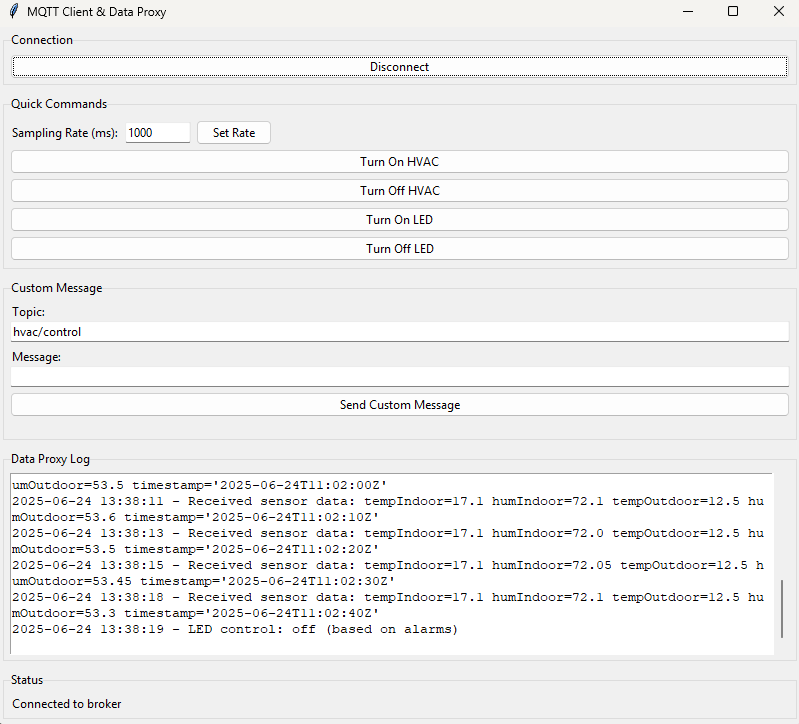
\includegraphics[width=1\linewidth]{image/data_proxy.png}
    \caption{Data proxy Tkinter interface}
    \label{fig:tkinter}
\end{figure}

For remote interaction, a \textbf{Telegram bot} allows mobile users to control and monitor the system without additional applications. The bot features a command-based interface with inline buttons, supports real-time status updates, and prevents unauthorized access through chat ID validation (Figure \ref{fig:telegram-bot}). 

\begin{figure}[H]\renewcommand{\thefigure}{6}
    \centering
    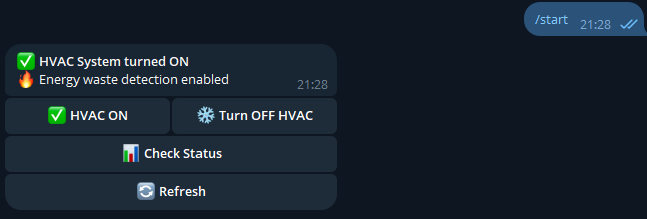
\includegraphics[width=1\linewidth]{image/telegram_bot.png}
    \caption{Telegram bot}
    \label{fig:telegram-bot}
\end{figure}

Finally, the system supports \textbf{Grafana} integration for advanced, customizable dashboards. These dashboards enable historical trend analysis and incorporate alerting mechanisms for waste detection.

\section{Results}

\begin{figure*}[t]\renewcommand{\thefigure}{10}
    \centering
    \begin{subfigure}[b]{0.48\linewidth}
        \centering
        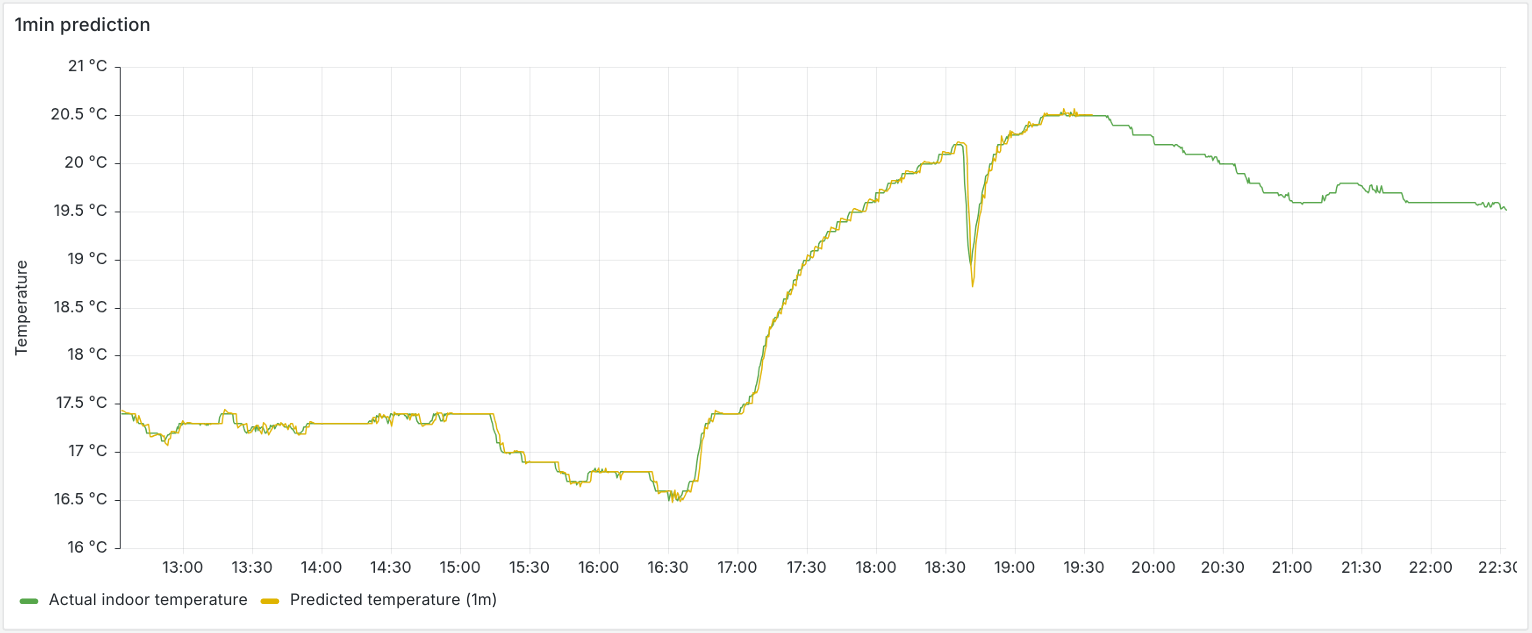
\includegraphics[width=\linewidth]{image/plot_1m_prediction.png}
        \caption{1-minute ahead prediction}
        \label{fig:prediction-1m-plot}
    \end{subfigure}
    \hfill
    \begin{subfigure}[b]{0.48\linewidth}
        \centering
        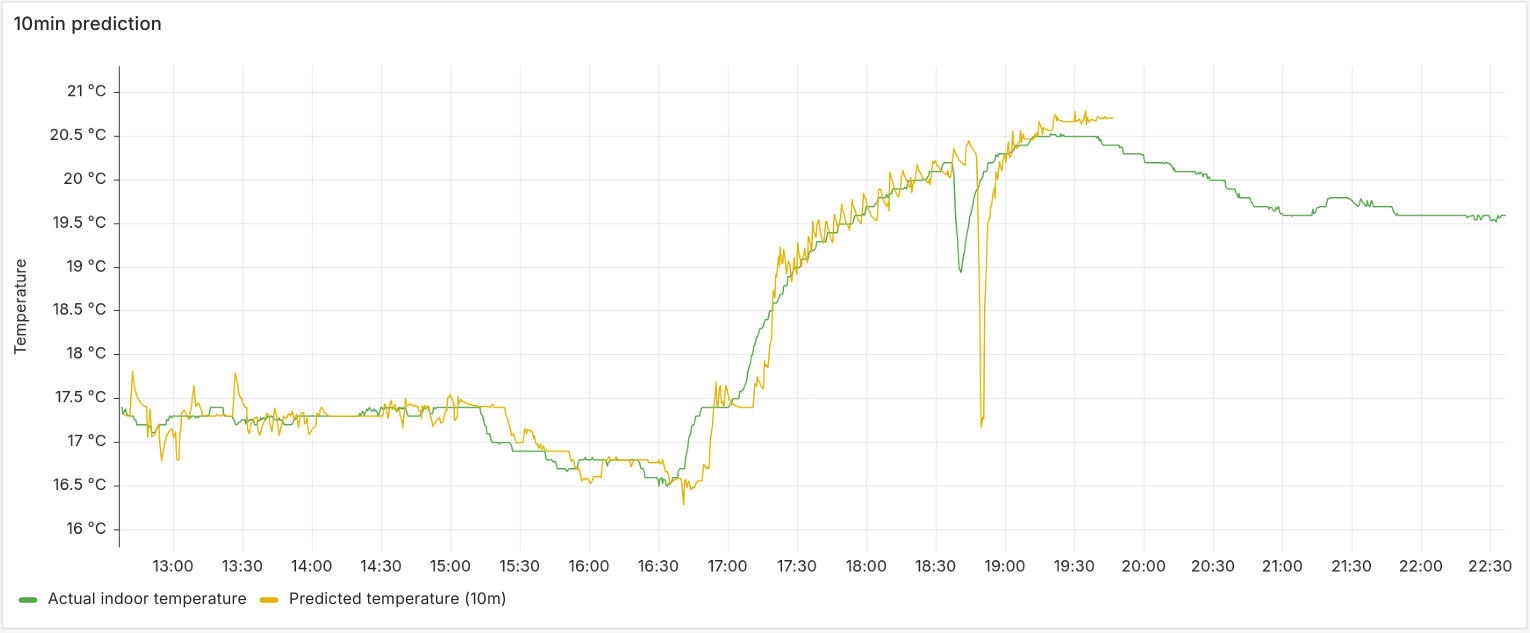
\includegraphics[width=\linewidth]{image/plot_10m_prediction.png}
        \caption{10-minute ahead prediction}
        \label{fig:prediction-10m-plot}
    \end{subfigure}
    \vspace{0.5cm}
    \begin{subfigure}[b]{0.48\linewidth}
        \centering
        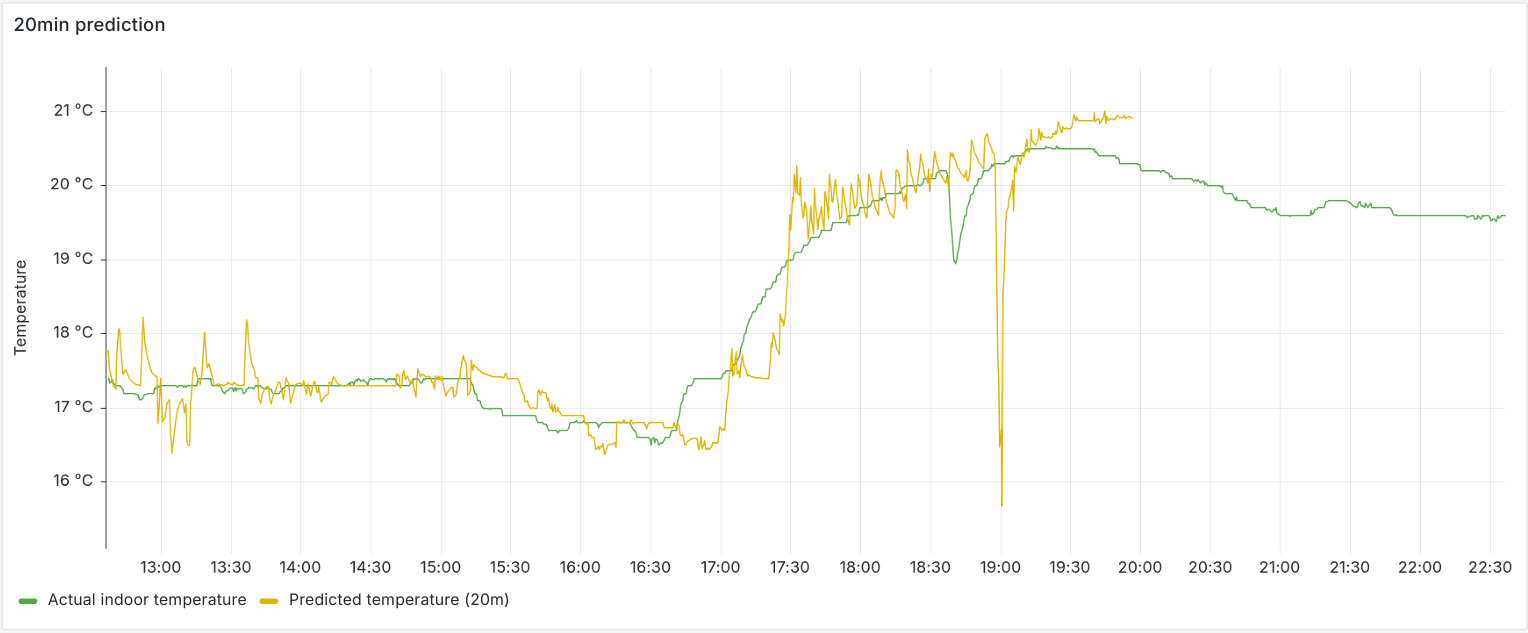
\includegraphics[width=\linewidth]{image/plot_20m_prediction.png}
        \caption{20-minute ahead prediction}
        \label{fig:prediction-20m-plot}
    \end{subfigure}
    \hfill
    \begin{subfigure}[b]{0.48\linewidth}
        \centering
        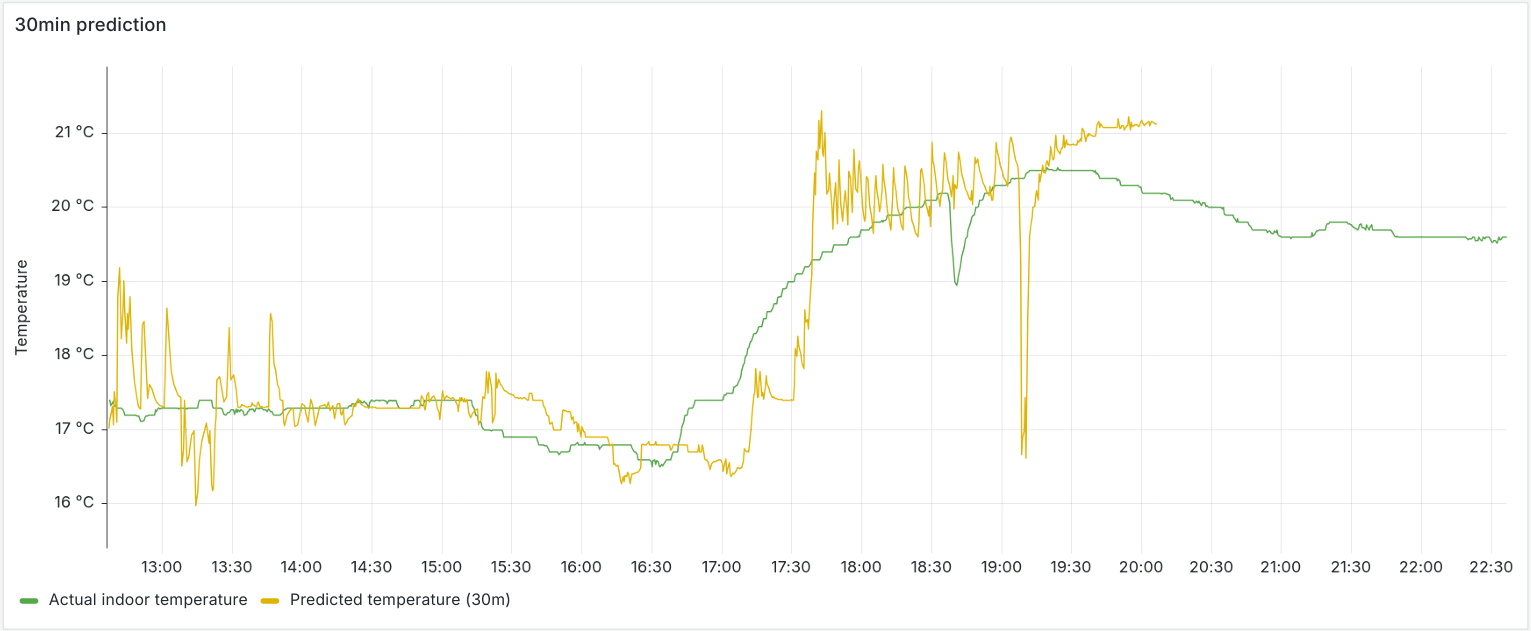
\includegraphics[width=\linewidth]{image/plot_30m_prediction.png}
        \caption{30-minute ahead prediction}
        \label{fig:prediction-30m-plot}
    \end{subfigure}
    \caption{Temperature forecasts at various time horizons}
    \label{fig:predictions-subfigures}
\end{figure*}

\begin{figure*}[!t]\renewcommand{\thefigure}{11}
    \centering
    \begin{subfigure}[b]{0.25\linewidth}
        \centering
        \includegraphics[width=\linewidth]{image/performance\_1m.png}
        \caption{1-minute prediction}
        \label{fig:prediction-performance-1m-plot}
    \end{subfigure}%
    \begin{subfigure}[b]{0.25\linewidth}
        \centering
        \includegraphics[width=\linewidth]{image/performance\_10m.png}
        \caption{10-minute prediction}
        \label{fig:prediction-performance-10m-plot}
    \end{subfigure}%
    \begin{subfigure}[b]{0.25\linewidth}
        \centering
        \includegraphics[width=\linewidth]{image/performance\_20m.png}
        \caption{20-minute prediction}
        \label{fig:prediction-performance-20m-plot}
    \end{subfigure}%
    \begin{subfigure}[b]{0.25\linewidth}
        \centering
        \includegraphics[width=\linewidth]{image/performance\_30m.png}
        \caption{30-minute prediction}
        \label{fig:prediction-performance-30m-plot}
        \end{subfigure}
        \caption{Forecasting performance at increasing prediction intervals}
    \label{fig:performance-subfigures}
\end{figure*}

This section presents the experimental results obtained from the IoT-based HVAC monitoring system. The following figures illustrate the system’s behavior during a representative 10-hour observation period, with data visualized using Grafana.

Figure \ref{fig:temperature-plot} displays the temperature readings collected from both the indoor and outdoor sensors over time. This plot provides an initial overview of the thermal dynamics captured by the system.

\begin{figure}[H]\renewcommand{\thefigure}{7}
    \centering
    \includegraphics[width=1\linewidth]{image/plot\_temperature.png}
    \caption{Indoor and outdoor temperature trends}
    \label{fig:temperature-plot}
\end{figure}

Figure \ref{fig:cumulative-alarm-plot} shows the cumulative number of HVAC waste alerts triggered per minute. This graph highlights the frequency and distribution of detected inefficiencies throughout the monitoring period.

\begin{figure}[H]\renewcommand{\thefigure}{8}
    \centering
    \includegraphics[width=1\linewidth]{image/plot\_cumulative\_alarm.png}
    \caption{Cumulative count of HVAC waste alerts per minute}
    \label{fig:cumulative-alarm-plot}
\end{figure}

In Figure \ref{fig:temperature-alarm-plot}, indoor and outdoor temperature trends are compared, with red highlights indicating instances where an HVAC waste condition was detected. This visualization enables direct correlation between temperature differentials and alert generation.

\begin{figure}[H]\renewcommand{\thefigure}{9}
    \centering
    \includegraphics[width=1\linewidth]{image/plot\_temperature\_with\_alarm.png}
    \caption{Temperature comparison with HVAC waste alert highlights}
    \label{fig:temperature-alarm-plot}
\end{figure}

The system generates temperature forecasts every 10 seconds. Each prediction is timestamped and stored in the database, with forecast horizons of 1, 10, 20, and 30 minutes. Figure \ref{fig:predictions-subfigures} illustrates the predictions generated at each of these horizons, plotted alongside the actual measured temperature values. For example, a prediction made at 14:00 for the 30-minute horizon is plotted against the real temperature recorded at 14:30, allowing visual evaluation of prediction accuracy.

For each stored forecast, performance metrics were computed using Mean Absolute Error (MAE), Mean Squared Error (MSE), and Root Mean Squared Error (RMSE). Figure \ref{fig:performance-subfigures} presents the model’s predictive performance across the four forecast intervals. As expected, shorter prediction horizons exhibit lower error values, while predictive accuracy deteriorates as the horizon extends.


Finally, Figure \ref{fig:latency-plot} presents the measured data transmission latency for each sensor reading. Latency is computed as the elapsed time between the message timestamp generated by the ESP32 and the final write operation to the InfluxDB database via the proxy. The average end-to-end latency is approximately 500 milliseconds, indicating near real-time processing capability.

\begin{figure}[H]\renewcommand{\thefigure}{12}
\centering
\includegraphics[width=1\linewidth]{image/plot\_latency.png}
\caption{Data transmission latency over time}
\label{fig:latency-plot}
\end{figure}

\subsection{Discussion of Results}
The temperature profiles depicted in Figure~\ref{fig:temperature-plot} reveal a clear correlation between indoor and outdoor conditions, with indoor temperatures exhibiting dampened fluctuations compared to outdoor ones. This behavior suggests effective thermal buffering by the indoor environment. The cumulative waste alerts shown in Figure~\ref{fig:cumulative-alarm-plot} occur primarily during significant temperature differentials, which is further confirmed by the direct overlay of alerts in Figure~\ref{fig:temperature-alarm-plot}. Thus, the system accurately identifies periods of potential energy inefficiency.

The predictive models demonstrate commendable short-term forecasting accuracy, as evinced by the low error values (MAE, MSE, and RMSE) for 1-minute ahead predictions in Figure~\ref{fig:performance-subfigures}. However, as forecast horizons extend to 30 minutes, the performance metrics deteriorate, reflecting increasing uncertainty intrinsic to longer-term predictions. Nonetheless, the system maintains an acceptable error margin for operational use within the first 10 minutes, enabling proactive HVAC control.

The observed average latency of approximately 500 ms (Figure~\ref{fig:latency-plot}) confirms that the end-to-end communication, spanning sensor reading, network transmission, proxy handling, and database storage—operates within the real-time constraints required for effective control action. This latency level supports timely forecast-driven adjustments and responsive alerting mechanisms.

Overall, the results validate the system’s capability to continuously monitor environmental conditions, generate reliable short-term forecasts, detect instances of energy waste, and maintain responsiveness compatible with real-time operational requirements.


\bibliographystyle{plain} % We choose the "plain" reference style
\bibliography{bibliography}

\end{document}
